\imprimirfolhaderosto*

%\includepdf{aprovacao.pdf}
%-----------------------------------------------%
% Inserir a ficha bibliografica %
%-----------------------------------------------%
% Isto é um exemplo de Ficha Catalográfica, ou ``Dados internacionais de
% catalogação-na-publicação''. Você pode utilizar este modelo como referência. 
% Porém, provavelmente a biblioteca da sua universidade lhe fornecerá um PDF
% com a ficha catalográfica definitiva após a defesa do trabalho. Quando estiver
% com o documento, salve-o como PDF no diretório do seu projeto e substitua todo
% o conteúdo de implementação deste arquivo pelo comando abaixo:
%
% \begin{fichacatalografica}
%     %\includepdf{fig_ficha_catalografica.pdf}    
% \end{fichacatalografica}

% ------------------------------
%EXEMPLO DE FICHA CATALOGRÁFICA
% ------------------------------
% \begin{fichacatalografica}
% 	\sffamily
% 	\vspace*{\fill}					% Posição vertical
% 	\begin{center}					% Minipage Centralizado
%         \fbox{
%             \begin{minipage}[c][8cm]{13.5cm}		% Largura
%                 \small
%                 \imprimirautor
%                 %Sobrenome, Nome do autor
                
%                 \hspace{0.5cm} \imprimirtitulo  / \imprimirautor. --
%                 \imprimirlocal, \imprimirdata-
                
%                 \hspace{0.5cm} \pageref{LastPage} p. : il. (algumas color.) ; 30 cm.\\
                
%                 \hspace{0.5cm} \imprimirorientadorRotulo~\imprimirorientador\\
                
%                 \hspace{0.5cm}
%                 \parbox[t]{\textwidth}{\imprimirtipotrabalho~--~\imprimirinstituicao,
%                 \imprimirdata.}\\
                
%                 \hspace{0.5cm}
%                     1. \firstkey.
%                     2. \secondkey.
%                     2. \thirdkey.
%                     I. Orientador.
%                     II. Universidade do Estado de Santa Catarina.
%                     III. \centro.
%                     IV. Título.
%             \end{minipage}
%         }
% 	\end{center}
% \end{fichacatalografica}
%-----------------------------------------------%

%-----------------------------------------------%
% Inserir folha de aprovação
%-----------------------------------------------%

% Isto é um exemplo de Folha de aprovação, elemento obrigatório da NBR
% 14724/2011 (seção 4.2.1.3). Você pode utilizar este modelo até a aprovação
% do trabalho. Após isso, substitua todo o conteúdo deste arquivo por uma
% imagem da página assinada pela banca com o comando abaixo:
%
% \includepdf{folhadeaprovacao_final.pdf}
 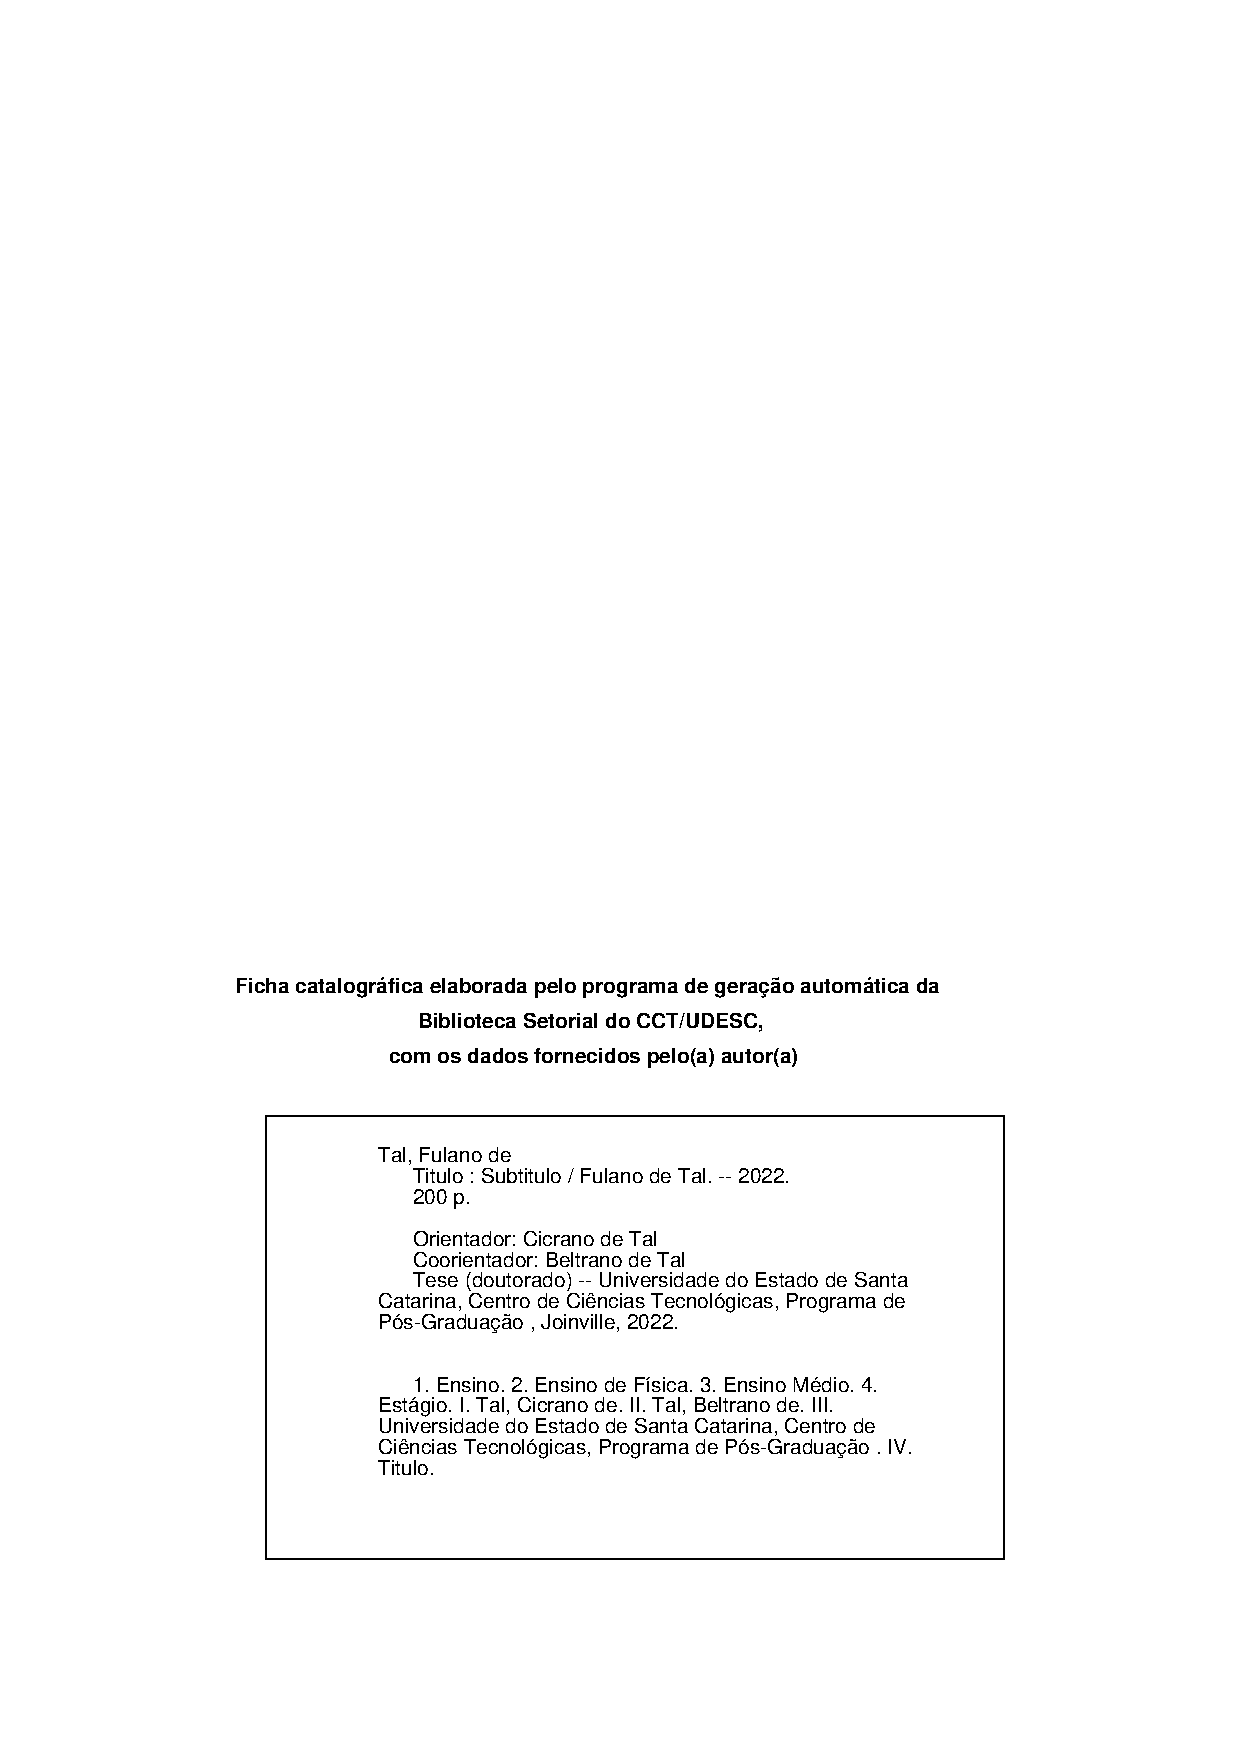
\includepdf[pages=-]{03-elementos/03.1_pre-textual/fichacatalografica.pdf}
%
\begin{folhadeaprovacao}
    \textoaprovacao{Este trabalho foi julgado adequado para obtenção do título de Engenheiro de Telecomunicações, pelo Instituto Federal de Educação, Ciência e Tecnologia de Santa Catarina, e aprovado na sua forma final pela comissão avaliadora abaixo indicada.}
    \begin{center}
        {\ABNTEXchapterfont\large\MakeUppercase{\imprimirautor}}

        \vspace*{\fill}\vspace*{\fill}
        \begin{center}
            \ABNTEXchapterfont\bfseries\Large\MakeUppercase{\imprimirtitulo}
        \end{center}
        \vspace*{\fill}
    
        \imprimirtextoaprovacao
     
        \vspace*{1cm}
    
	    \imprimirlocal, 6 de maio de 2021:

    \vspace*{\fill}
   \end{center}
        


   \assinatura{\textbf{\imprimirorientador} \\ Orientador\\Instituto Federal de Santa Catarina} 
   \assinatura{\textbf{Professor Fulano, Dr.} \\ Instituto X }
   \assinatura{\textbf{Professora Fulana, Dra. } \\ Instituto Y}
   \assinatura{\textbf{Professor Beltrano, Dr.} \\ Instituto Z}
   \assinatura{\textbf{Professor} \\ Convidado 4}
      
    \vspace*{1cm}  
  
\end{folhadeaprovacao}
%-----------------------------------------------%